% MS&E 226 Project Part 1 report template
% Handout limits: <= 5 pages of text, >= single spaced, 11pt Times, >= 1in margins,
% plus at most 1 extra page for figures only.
% Red \TODO notes are placeholders. Delete each one when filled.
% To hide every TODO before submitting, change \showtodostrue to \showtodosfalse.
\documentclass[11pt]{article}
\usepackage[margin=1in]{geometry}
\usepackage{mathptmx}            % Times
\usepackage[T1]{fontenc}
\usepackage{booktabs,tabularx,graphicx,xcolor,enumitem}
\usepackage[hidelinks]{hyperref}
\setlist{nosep,leftmargin=*}
\setlength{\parskip}{3pt}\setlength{\parindent}{0pt}

\newif\ifshowtodos \showtodostrue
\newcommand{\TODO}[1]{\ifshowtodos{\color{red}\textbf{[TODO: #1]}}\fi}

\title{\vspace{-1.5cm}MS\&E 226 Project Part 1: Predicting Nursing Home Inspection Deficiencies}
\author{Emily \TODO{last name} \and Alex \TODO{last name} \and Evy Shen}
\date{November 2026}

\begin{document}
\sloppy
\maketitle
\vspace{-1cm}

% ======================================================================
\section{Stakeholder presentation preparation}
\textbf{(a) Stakeholder.} \TODO{Emily: confirm or replace. Draft:}
Our stakeholder is a \emph{state survey agency}, the state office that inspects nursing homes on behalf of the Centers for Medicare \& Medicaid Services (CMS). Each agency must complete standard surveys on every certified facility with a limited number of inspectors. It would commission this analysis to decide which facilities to inspect first, or more closely, given its limited staff time.

\textbf{(b) Decision and timing.} The model predicts how many health deficiencies a facility will receive at its next standard inspection. The prediction is made \emph{before} the inspection is scheduled. At that point the agency has the facility's profile (ownership, size, chain membership, location), its self-reported staffing and turnover, its resident case mix, and the results of its \emph{earlier} inspections. Nothing from the upcoming inspection is available, so every variable derived from it is excluded (Section 3). The agency would rank facilities by predicted deficiencies and prioritize the top of the list. \TODO{Emily: one-line rule for what counts as known at prediction time.}

% ======================================================================
\section{Outcome}
The outcome is \texttt{Rating Cycle 1 Total Number of Health Deficiencies}: the number of health deficiencies cited at a facility's most recent standard inspection. It is continuous in practice (a count from 0 to 84 in the development data, median 7, mean 9.2), and it maps directly onto the agency's question of where violations are likely. We chose it over \texttt{Overall Rating} because CMS computes the overall rating from the inspection, staffing and quality-measure ratings. Predicting it would mostly recompute CMS's formula, and removing those inputs to avoid leakage leaves an incoherent story. The outcome is right-skewed, so we also consider $\log(1+Y)$ as a transformation in one feature set (Section 6). \TODO{Emily: confirm the outcome choice.}

% ======================================================================
\section{Dataset}
\textbf{(a) Eligibility.} Source: CMS Provider Data Catalog, ``Nursing Homes Including Rehab Services: Provider Information,'' processing date 2026-10-01 (\url{https://data.cms.gov/provider-data/dataset/4pq5-n9py}). These are publicly released U.S.\ government data. \TODO{Emily: confirm the terms of use on the CMS site and state permission.}
\begin{enumerate}[label=(\roman*)]
  \item 14{,}686 rows; one row is one Medicare/Medicaid-certified nursing home (identified by its CMS Certification Number). There are 102 columns, of which we use 24 (feature set 1) or 35 (feature set 2) as predictors (Section 6d).
  \item Predictors are both numeric (beds, staffing hours per resident-day, turnover, case-mix index) and categorical (ownership type, state, urban/rural, provider type, chain membership).
  \item The data are real administrative records: inspection results and payroll-based staffing reports, not simulated.
  \item The file is a single snapshot with one row per facility, not a time series or panel. Date columns are not used as features; \texttt{Date First Approved} may be converted to ``years certified,'' analogous to house age. \TODO{decide}
  \item Missingness is modest for the variables we use: about 3\% for staffing, 7--13\% for turnover, and 0.3\% (31 rows) for the outcome. The 24 columns that are more than 30\% missing are almost all footnote codes, which we drop.
\end{enumerate}
\emph{Independence caveat:} 69\% of development facilities belong to one of 611 chains (the largest has 284 development rows). Facilities in a chain share management, so rows are not perfectly independent. We treat facilities as independent units and assess the impact in Section 6(b).

\textbf{(b) Description and fit.} \TODO{Emily: 3--4 sentences.} The data cover essentially every certified nursing home in the U.S., which is the agency's own population of facilities. They contain the operational signals an agency already has before an inspection: staffing levels, staff turnover, resident acuity, ownership and chain affiliation. They also include prior inspection results, which lets us measure how much inspection history adds over facility characteristics alone.

\textbf{(c) Duplicates.} We checked for exact duplicate rows, duplicate CMS Certification Numbers, and duplicate name\,+\,address\,+\,city\,+\,state combinations. None were found, so all 14{,}686 rows were kept (\texttt{01\_dedup\_and\_split.py}).

% ======================================================================
\section{Holdout set}
Before any exploration, we randomly set aside 20\% of facilities as a holdout using \texttt{train\_test\_split} with seed \textbf{226}. This gives \textbf{11{,}748} development rows and \textbf{2{,}938} holdout rows. The script pins SHA-256 fingerprints of the raw file and of the holdout's facility IDs, and saves every facility's assignment (\texttt{split\_ccns.csv}), so the split is exactly reproducible. One team member keeps \texttt{holdout.csv} outside all shared folders. It is never opened, committed to our repository (\texttt{.gitignore} blocks all data), or given to AI tools until Part 2. \TODO{Honest note: the file briefly sat in a shared folder given to an AI assistant, which did not open it, and it was then moved. Keep or reword.}

% ======================================================================
\section{Data description and exploration}
\textbf{(a) Data collection.} \TODO{Alex: how CMS collects inspections (state surveyors, standard vs.\ complaint surveys), self-reported Payroll-Based Journal staffing, how ratings are computed; issues: self-reporting, inspection dates from 2019 to 2026, differences in inspector strictness across states.}

\textbf{(b) Correlations with the outcome.} \TODO{Alex. Preliminary Spearman correlations on the development data: prior-cycle health score 0.50, total nursing turnover 0.22, certified beds 0.19, total nurse staffing hours $-0.19$, case-mix index 0.11. Include plots (Figure~1).}

\textbf{(c) Correlations among covariates.} \TODO{Alex: e.g., the reported, case-mix and adjusted staffing measures are near-duplicates; beds vs.\ residents per day.}

\textbf{(d) Subgroups.} \TODO{Alex: ownership (for-profit / non-profit / government), chain vs.\ independent, state, urban/rural.}

\textbf{(e) Missing values.} \TODO{Alex: drop footnote columns; median or most-frequent imputation fit inside each CV training fold (and missing-indicator columns?); drop the 31 rows with a missing outcome.}

% ======================================================================
\section{Prediction}
\textbf{(a) Metrics.} The primary metric is \textbf{RMSE} (in deficiencies), from 5-fold cross validation. RMSE is in the agency's units (``predictions are off by about $X$ deficiencies'') and penalizes large misses most. Large misses are the facilities an agency most needs to catch. Secondary metrics: MAE (typical error, less sensitive to the skewed tail) and Spearman rank correlation between predicted and actual counts, which measures how well the model \emph{orders} facilities for prioritization. \TODO{Emily: confirm the primary metric.}

\textbf{(b) Training and comparison procedure.} All work uses only the 11{,}748 development rows. We use 5-fold \texttt{KFold(shuffle=True, random\_state=226)}. One fold object is created once and reused by every algorithm and feature set, so all comparisons use identical splits. Imputation, one-hot encoding and standardization are wrapped in an sklearn \texttt{Pipeline} and fit only on each training fold, then applied to the validation fold. Feature engineering (ratios, logs, facility age) is row-wise and uses only fixed constants, so it introduces no cross-fold information. Tuned models use \emph{nested} CV: inside each outer training fold, \texttt{GridSearchCV} picks hyperparameters on 3 inner folds (seed 226), and the tuned model is scored on the untouched outer fold. Tuning on the reported folds themselves would give an optimistically biased score (the ``winner's curse''). Because 69\% of facilities belong to chains, we also refit the FS2 models on chain-grouped folds (\texttt{GroupKFold}; independents form their own groups). Grouped CV raised RMSE by only 0.03--0.07 and did not change the ranking of models, so plain CV is slightly optimistic but adequate for model selection. The feature sets were motivated by exploratory analysis of the full development data, which makes CV estimates slightly optimistic; the untouched holdout gives the unbiased estimate in Part 2.

\textbf{(c) Baseline.} We predict the training-fold mean deficiency count for every facility, which is the constant that minimizes squared error. Its CV RMSE is \textbf{8.07} deficiencies (MAE 5.87). Beating it shows that facility information carries signal beyond the national average; the size of the improvement tells the agency how much better prioritization becomes.

\textbf{(d) Algorithms and feature sets.}
\begin{itemize}
  \item \textbf{OLS linear regression:} minimizes squared error over linear functions of the features. It is interpretable and unbiased under a linear model, but it has no defense against variance from many correlated features. \TODO{Alex}
  \item \textbf{Lasso:} squared error plus $\lambda\sum_j|\beta_j|$ on standardized features. It trades some bias for lower variance and sets weak coefficients to exactly zero, which helps with near-duplicate columns (weekday vs.\ weekend staffing, several history scores). We preferred it to ridge for that shorter, more explainable feature list. Penalty: 30 log-spaced values of sklearn's $\alpha=\lambda/2n$ from $10^{-4}$ to $1$.
  \item \textbf{Random forest:} averages many regression trees, each grown greedily on a bootstrap sample with random feature subsets at each split. It captures nonlinearities and interactions (for example, staffing effects that differ by size or ownership); averaging reduces the high variance of single trees. We chose it over gradient boosting because it has fewer hyperparameters that matter. Grid: max depth $\{\mathrm{none}, 15\}$ $\times$ min samples per leaf $\{1,5,20\}$ $\times$ features per split $\{\sqrt{p}, 0.33p\}$ (12 settings, 300 trees, seed 226).
\end{itemize}
\emph{Feature set 1 (facility profile):} ownership (collapsed to three levels), urban/rural, provider type, in-hospital, CCRC, beds, residents per day, chain membership and chain size, reported staffing hours (RN, LPN, aide, total, weekend, PT), turnover (nursing, RN, administrator), case-mix index, ownership change in the last 12 months, resident \& family council, sprinklers, state. \\
\emph{Feature set 2 (profile + history + engineered):} Set 1 plus prior-cycle inspection results (\texttt{Rating Cycle 2/3} counts and scores), occupancy (residents/beds), RN share of nursing hours, years certified, and $\log$(beds). This set tests how much inspection history and nonlinear transformations add.\\
\emph{Excluded for leakage:} every \texttt{Rating Cycle 1} column, \texttt{Total Weighted Health Survey Score}, health-inspection and overall ratings (including chain averages), abuse, special-focus and high-performing icons, the ``inspection more than 2 years ago'' flag, and fines, penalties and payment denials. The staffing rating (computed from the included staffing hours) and the QM ratings (another CMS rating) are also excluded. \TODO{Alex/Emily: confirm the feature sets.}

\textbf{(e) Results.}
\begin{table}[h]\centering\small
\begin{tabularx}{\linewidth}{llcccX}
\toprule
Algorithm & Set & RMSE (mean $\pm$ SD) & MAE & Spearman & Tuning tried $\rightarrow$ selected (5 outer folds) \\
\midrule
Baseline (mean) & -- & 8.065 $\pm$ 0.176 & 5.870 & -- & -- \\
OLS & 1 & 6.649 $\pm$ 0.179 & 4.729 & 0.587 & none \\
OLS & 2 & 5.912 $\pm$ 0.112 & 4.207 & 0.671 & none \\
Lasso & 1 & 6.649 $\pm$ 0.179 & 4.727 & 0.586 & 30 $\alpha$ values $\rightarrow$ 0.0013--0.0024 \\
\textbf{Lasso} & \textbf{2} & \textbf{5.904 $\pm$ 0.104} & \textbf{4.199} & \textbf{0.671} & 30 $\alpha$ values $\rightarrow$ 0.0017--0.0033 \\
Random forest & 1 & 6.620 $\pm$ 0.149 & 4.754 & 0.566 & 12 settings $\rightarrow$ no depth limit, leaf 1, $\sqrt{p}$ (4 of 5 folds) \\
Random forest & 2 & 6.031 $\pm$ 0.086 & 4.332 & 0.642 & 12 settings $\rightarrow$ no depth limit, leaf 1, $\sqrt{p}$ (5 of 5 folds) \\
\bottomrule
\end{tabularx}
\caption{Nested 5-fold CV on the 11{,}717 development rows with a non-missing outcome (identical outer folds, seed 226). RMSE and MAE are in deficiencies. Spearman is the rank correlation between predicted and actual counts. Total tuning: 30 lasso and 12 random-forest settings per feature set, each tried on 3 inner folds within all 5 outer folds.}
\end{table}
\vspace{-0.3cm}
Every model beats the baseline by a wide margin. The best models cut RMSE by about 27\% (8.07 to 5.90), which explains roughly 46\% of the variance out of fold. \emph{Feature set matters more than algorithm:} adding prior inspection history and the engineered features (set 2) lowers RMSE by about 0.74 deficiencies for the linear models and 0.59 for the random forest. That gain is 4--7 times the fold-to-fold SD and lifts the rank correlation from about 0.59 to 0.67, a real improvement in how well the agency can order facilities. \emph{Within a feature set, algorithms are nearly tied.} Lasso and OLS differ by 0.008 RMSE, and their per-fold differences change sign. The selected penalties are small because $n=11{,}717$ is large relative to about 105 encoded columns, so OLS variance is already low. The random forest ties the linear models on set 1 but is worse on set 2 (by 0.13, in all 5 folds). Its strongest signal, prior deficiencies, is close to linear, so the forest's flexibility adds variance without reducing bias. Two checks confirm this. Pushing the forest beyond its grid edge ($0.1p$, $0.5p$, $p$ features per split) gave 6.03--6.10, and an untuned gradient-boosting model reached 5.94, close to lasso but not better. For the agency, a 0.1-deficiency gap between algorithms is not practically meaningful; including inspection history is.

\textbf{(f) Final model.} We select \textbf{lasso on feature set 2}. It has the lowest CV RMSE, the primary metric. It is statistically tied with OLS, but its shrinkage stabilizes the collinear staffing and history columns, and it was the least optimistic model under chain-grouped CV (+0.03). Unlike the forest, its coefficients can be explained to the agency. Refit on all development data, CV re-selects $\alpha=0.0024$ (84 of 105 coefficients nonzero; non-nested CV RMSE 5.905). Holding other features fixed, \emph{associations} (not causal effects) per standard deviation:
\begin{itemize}
  \item Prior-cycle deficiencies: $+5.0$, by far the strongest predictor.
  \item Facility size ($+0.9$ per SD of log beds), a recent ownership change ($+0.8$), and administrator, RN and nursing turnover ($+0.5$ each).
  \item Total nurse staffing hours: $-0.4$. Non-profit ($-0.6$) and government ($-0.5$) ownership predict fewer deficiencies than for-profit.
  \item State effects are large (40 of 52 state indicators are nonzero) and likely reflect inspector strictness as well as care quality.
\end{itemize}
The fitted pipeline (imputation, encoding, scaling, lasso) is saved by \texttt{scripts/04\_final\_model.py} as \texttt{models/final\_pipeline.joblib}. There is no classification threshold. It will be scored once on the holdout in Part 2.

% ======================================================================
\section{Stakeholder guidance}
\textbf{(a) Decisions supported.} \TODO{Emily: e.g., ranking facilities for inspection priority; performance in plain terms; further evidence needed before acting (holdout evaluation in Part 2, a pilot comparing model-guided and usual scheduling).}

\textbf{(b) Limitations.} \TODO{Emily: correlation is not causation (low staffing predicts deficiencies, but the model does not show that adding staff reduces them); deficiency counts also reflect inspector strictness by state; staffing data may postdate the inspection; chain clustering; the model may be unreliable for unusual facilities (hospital-based, very small); fairness across ownership types.}

% ======================================================================
\section{AI tools}
\TODO{Each member: tools and versions, tasks delegated, how outputs were checked, one concrete suggestion accepted/modified/rejected.}
Evy used Claude (Anthropic, Claude Opus 5.5, Claude desktop app). It summarized lecture slides, planned the work split, reviewed the split script, recommended an outcome and leakage list, and wrote the Section 6 code (shared pipeline, nested CV, robustness checks, final model) and a first draft of Sections 6b--6f. Checks: \TODO{Evy: e.g., reran the scripts from a clean clone, confirmed no code reads the holdout, spot-checked the leakage list against the CMS rating methodology, and checked that every number in Table 1 matches \texttt{results/cv\_results.csv}.} Example: \TODO{Evy: e.g., the assistant first planned to tune on the same folds it reported; we modified this to nested CV so the tuned models' scores are not optimistic.}

% ======================================================================
\section{Code}
Code (data split, preprocessing, feature construction, model selection, final pipeline, seeds, package versions and data-access instructions): \TODO{Stanford Drive link to code zip}. Repository: \TODO{GitHub URL}. Data are not included; see \texttt{data/README.md} for download instructions.

% ======================================================================
\clearpage
\section*{Figures}
\TODO{Up to one page of figures: outcome distribution, top correlations, subgroup boxplots.}
% 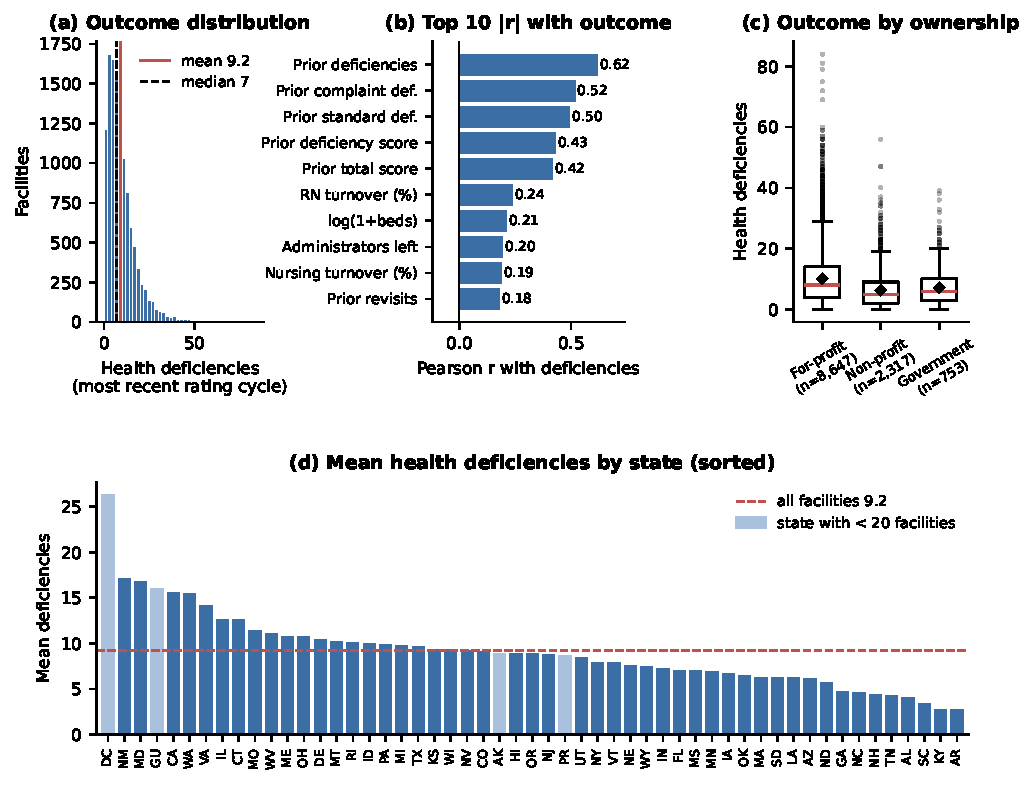
\includegraphics[width=\linewidth]{figures/fig1.pdf}

\end{document}
